\documentclass{beamer}
\usetheme[faculty=med]{fibeamer}
\usepackage[utf8]{inputenc}
\usepackage[
  main=english
]{babel}        %% typeset as follows:
%% These macros specify information about the presentation
\title{Algoritmos} %% that will be typeset on the
\subtitle{Introdução} %% title page.
\author{Guilherme Meira}
%% These additional packages are used within the document:
\usepackage{ragged2e}  % `\justifying` text
\usepackage{booktabs}  % Tables
\usepackage{tabularx}
\usepackage{tikz}      % Diagrams
\usetikzlibrary{calc, shapes, backgrounds, positioning}
\usepackage{minted}
\usepackage{amsmath, amssymb}
\usepackage{url}       % `\url`s
\usepackage{listings}  % Code listings
\usepackage{xcolor}
\definecolor{highlightcolor}{RGB}{255, 140, 119}
\setminted{highlightcolor=highlightcolor}
\frenchspacing
\begin{document}
  \frame{\maketitle}
  \AtBeginSection[]{% Print an outline at the beginning of sections
  	\begin{frame}<beamer>
  		\frametitle{Agenda}
  		\tableofcontents[currentsection]
  	\end{frame}}
  	
  \begin{frame}{Primeiramente...}
	\begin{tikzpicture}[overlay,remember picture]
		\node at (current page.center) {
			
\includegraphics[width=0.7\paperwidth]{resources/why}
		};
	\end{tikzpicture}
  \end{frame}
  \begin{frame}{Primeiramente...}
  	\begin{tikzpicture}[overlay, remember picture, node distance=0]
  	\node[anchor=center] (dif1) at (current page.center) {
  		
\includegraphics[width=0.3\paperwidth]{resources/different2}
  	};
  	\node[left=of dif1, yshift=30pt] {
  		
\includegraphics[width=0.3\paperwidth]{resources/different1}
  	};
  	\node[right=of dif1, yshift=-20pt] {
  		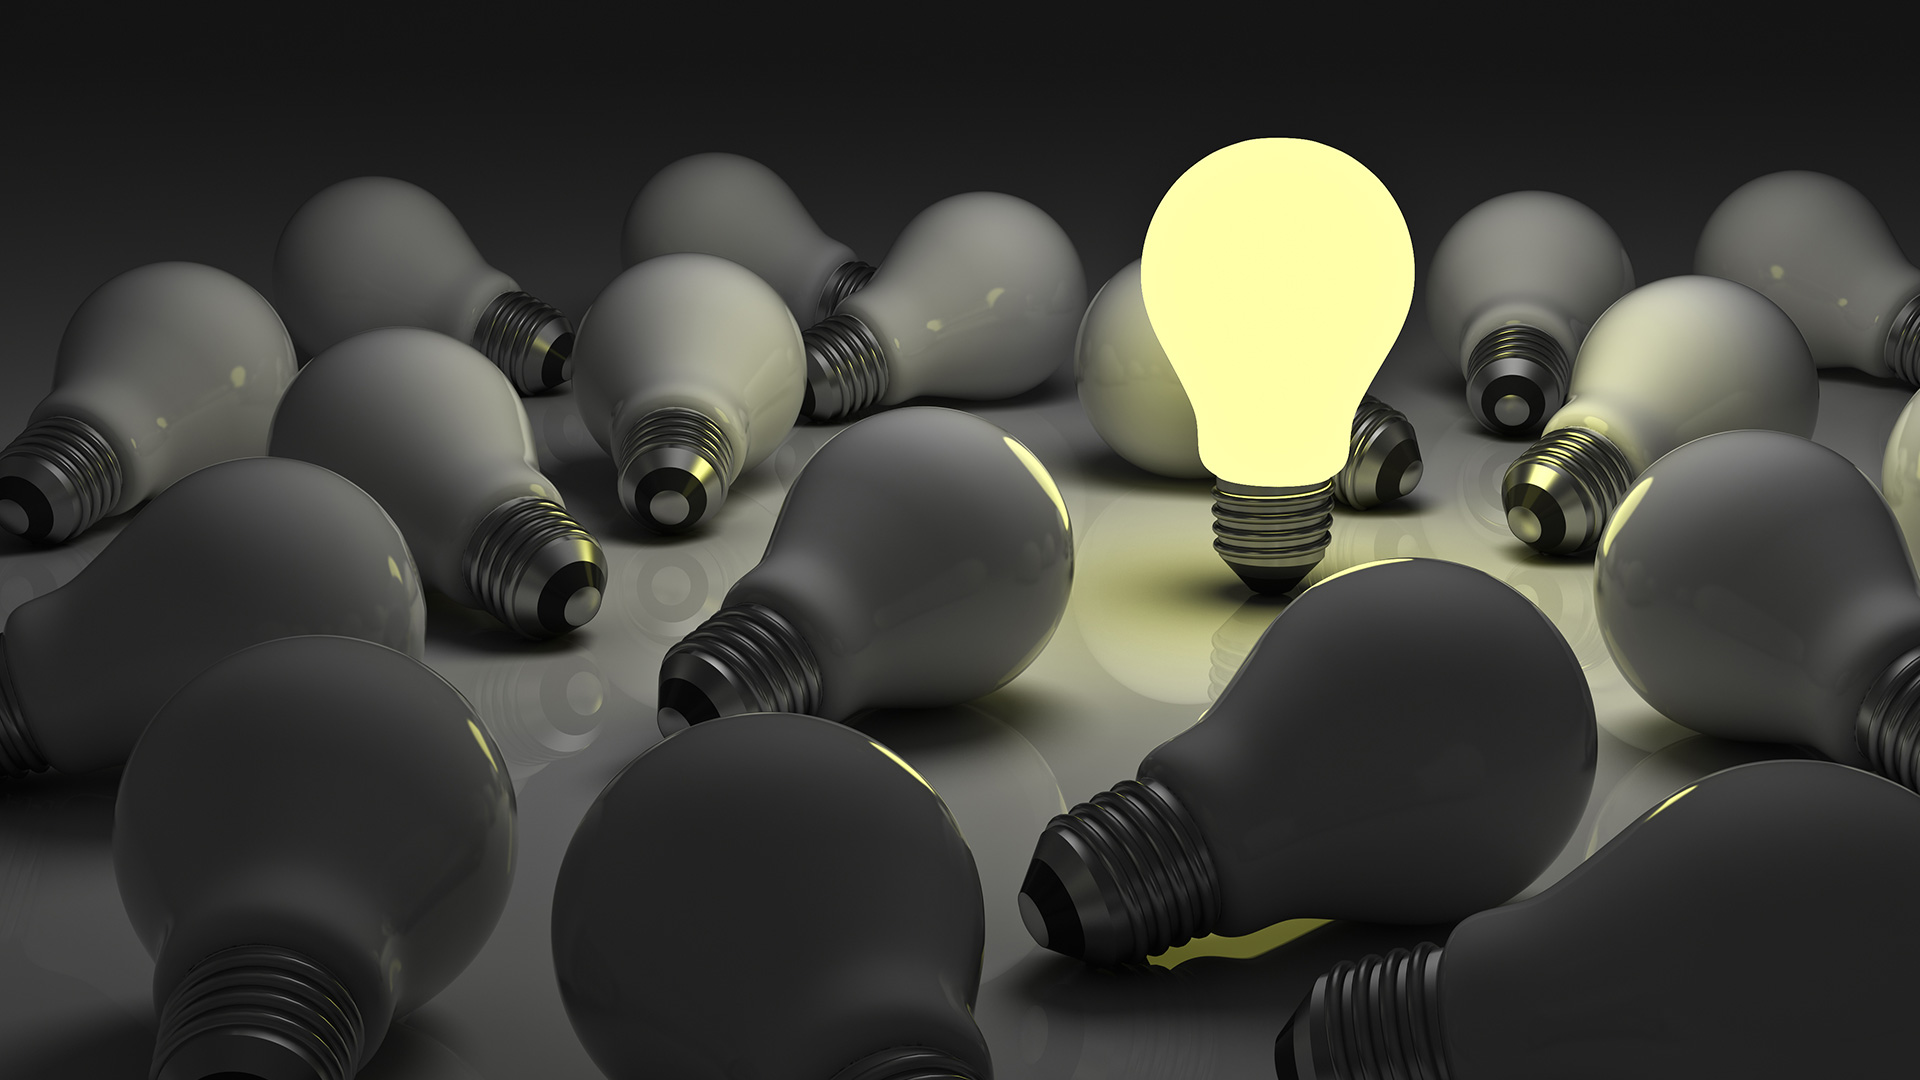
\includegraphics[width=0.3\paperwidth]{resources/different3}
  	};
  	\pause
   	\node[anchor=center] at (current page.center) {
   		
\includegraphics[width=0.8\paperwidth]{resources/lazy}
   	};
  	\end{tikzpicture}
  \end{frame}
  \begin{frame}{Primeiramente...}
  	\begin{tikzpicture}
	  	\node at (current page.center) {
	  		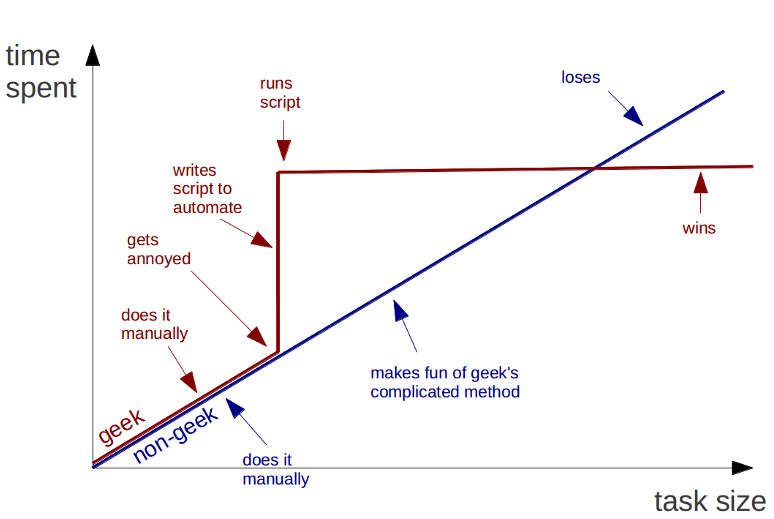
\includegraphics[width=0.8\paperwidth]{resources/automation}
	  	};
  	\end{tikzpicture}
  \end{frame}
  \begin{frame}{Primeiramente...}
  	\begin{itemize}
	    \item<1-> Tarefas repetitivas
	    \item<2-> Matemática
	    	\begin{equation*}
	    	\int_0^\infty e^{-ax^2}(1+x^2)^{z-1/2}\cos(2ax+(2z-1)\tan^{-1}(x))\,\mathrm{d}x
	    	\end{equation*}
	    \item<3-> Estatística
	    \item<4-> Formatura
	  \end{itemize}
	  \begin{tikzpicture}[overlay, remember picture]
	  \node[anchor=north east, yshift=-20, xshift=-20] at (current page.north east) {
	  	
\includegraphics[width=0.3\paperwidth]{resources/boring}
	  };
	  \node<3->[anchor=south east, yshift=20, xshift=-20] at (current page.south east) {
	  	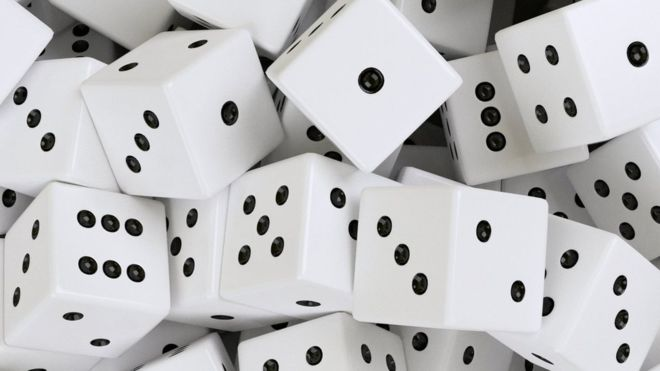
\includegraphics[width=0.3\paperwidth]{resources/dice}
	  };
	  \node<4->[anchor=south east, yshift=20, xshift=20] at (current page.south) {
	   	
\includegraphics[width=0.2\paperwidth]{resources/troll}
	  };
	  \end{tikzpicture}
  \end{frame}
  \section{Apresentação da disciplina}
  \begin{frame}{Apresentação da disciplina}
  	\begin{itemize}
  		\item[Disciplina] Algoritmos
  		\item[Professor] Guilherme Meira
	  	\item[Horário] Segundas-feiras, das 18:50h às 22:00h
		  	\begin{itemize}
		  		\item Intervalo de 10 minutos por volta das 20:20h
		  		\item Chamada ao final da aula
		  	\end{itemize}
		\item[Avaliação] Duas provas + listas de exercício
			\begin{itemize}
				\item 7 pontos de prova ($P_{1}$ e $P_{2}$)
				\item 3 pontos de listas de exercício ($T_{1}$ e $T_{2}$)
				\item $M_{P} = \frac{P_{1} + T_{1} + P_{2} + T_{2}}{2}$
				\item $M_{P} \ge 7$: aprovado
				\item $M_{P} < 7$: prova final ($P_{F}$)
				\item $M_{F} = \frac{M_{P} + P_{F}}{2}$
				\item $M_{F} \ge 5$: aprovado
				\item $M_{F} < 5$: gostou  tanto da matéria que vai fazer de novo
			\end{itemize}
  	\end{itemize}
  \end{frame}
  \begin{frame}{Apresentação da disciplina}
  	\begin{itemize}
	  	\item[Trabalhos] Exercícios práticos de programação
		  	\begin{itemize}
		  		\item Individual
		  		\item Aproximadamente a cada 2 semanas
		  		\item Correção automática
		  	\end{itemize}
		\item[Livros] Há muito material disponível na internet
			\begin{itemize}
				\item Livros da bibliografia do curso
				\item C Completo e Total (7 exemplares na biblioteca)
			\end{itemize}
		\item[Outros]
			\begin{itemize}
				\item Honestidade acadêmica
				\item Comportamento em sala
				\item Feedback!
			\end{itemize}
	\end{itemize}
  \end{frame}
  
  \section{Introdução}
  \begin{frame}{Introdução}
  	\framesubtitle{O que é um Algoritmo?}
	\begin{block}{Definição}<2->
		Um \alert{algoritmo} é uma especificação não-ambígua de como resolver uma classe de problemas.
	\end{block}
	\begin{tikzpicture}[overlay, remember picture]
		\node<3->[anchor=north east, yshift=-20, xshift=-20] at (current page.north east) {
			
\includegraphics[width=0.3\paperwidth]{resources/sir}
		};
	\end{tikzpicture}
  \end{frame}
  \begin{frame}{Introdução}
  	\framesubtitle{O que é um Algoritmo?}
  	Exemplo:
  	\begin{itemize}
  		\item[Problema] Fazer bolo
  		\item[Algoritmo]
  		\begin{itemize}
  			\item Bata as claras em neve e reserve
  			\item Misture as gemas, a margarina e o açúcar até obter uma massa homogênea
  			\item Acrescente o leite e a farinha de trigo aos poucos, sem parar de bater
  			\item Por último, adicione as claras em neve e o fermento
  			\item Despeje a massa em uma forma grande de furo central untada e enfarinhada
  			\item Asse em forno médio 180 °C, preaquecido, por aproximadamente 40 minutos ou ao furar o bolo com um garfo, este saia limpo
  		\end{itemize}
  	\end{itemize}
  \end{frame}
  \begin{frame}{Introdução}
	\framesubtitle{O que é um Algoritmo?}
	Exemplo:
	\begin{itemize}
		\item[Problema] Calcular as raízes da equação $a\cdot x^{2} + b\cdot x + c = 0$
		\item[Algoritmo]
		\begin{itemize}
			\item Calcular o valor de $\Delta = b^{2} - 4\cdot a\cdot c$
			\item Usar o valor de delta para calcular as raízes:
			\begin{equation*}
				x = -\frac{b^{2}\pm \sqrt{\Delta}}{2\cdot a}
			\end{equation*}
		\end{itemize}
	\end{itemize}
	\pause
	Queremos ensinar ao computador como resolver tarefas por meio de algoritmos.
  \end{frame}
  \begin{frame}{Introdução}
  	\framesubtitle{Como ensinar um computador?}
  	Computadores são capazes de executar pequenas tarefas chamadas de \alert{instruções}.
  	
  	Devemos descrever algoritmos por meio de uma sequência de instruções que o computador é capaz de executar.
  	
  	\only<1>{
  		\begin{figure}
	  		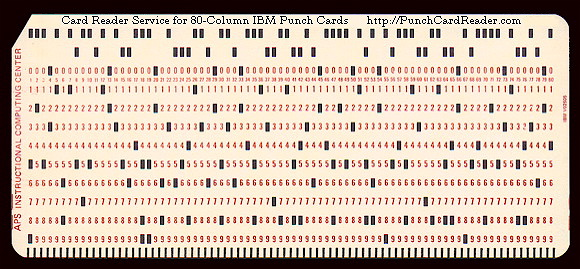
\includegraphics[width=0.5\paperwidth]{resources/punchcard}
	  	\end{figure}
	}
	\only<2>{
		\begin{figure}
			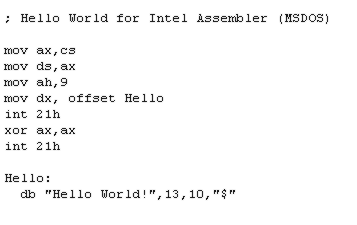
\includegraphics[width=0.5\paperwidth]{resources/assembly}
		\end{figure}
	}
	\only<3>{
		\begin{figure}
			
\includegraphics[width=0.4\paperwidth]{resources/languages}
		\end{figure}
	}
  \end{frame}
  \begin{frame}{Introdução}
  	\framesubtitle{Como ensinar um computador?}
  	\begin{center}
	  	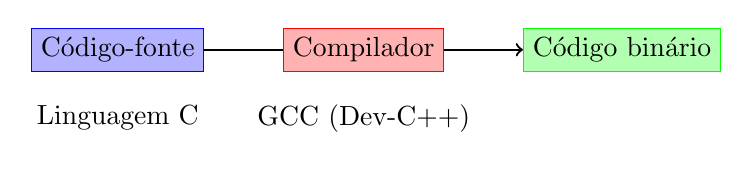
\begin{tikzpicture}[node distance=3mm and 1cm]
	  	\centering
	  	\node[draw=blue, fill=blue!30] (fonte) at (0,0) {Código-fonte};
	  	\node[draw=red, fill=red!30, right=of fonte] (compilador) {Compilador};
	  	\node[draw=green, fill=green!30, right=of compilador] (binario) {Código binário};
	  	\draw[->, thick] (fonte) -- (compilador) -- (binario);
	  	
	  	\pause
	  	
	  	\node[below=of fonte] {Linguagem C};
	  	\node[below=of compilador] {GCC (Dev-C++)};
	  	\end{tikzpicture}
	\end{center}
  \end{frame}
  \begin{frame}{Introdução}
  	\framesubtitle{Linguagem C}
  	\begin{itemize}
  		\item Desenvolvida por Dennis Ritchie entre 1969 e 1973
  		\item Presente em \textbf{muitas} plataformas
  		\item Baixo nível
  		\item Utilizam C:
	  		\begin{itemize}
	  			\item Sistemas operacionais (Windows, Linux)
	  			\item Jogos (Doom, Quake)
	  			\item Bancos de dados (MySQL, Oracle)
	  			\item Linguagens de programação (Python, Ruby)
	  			\item Muitos outros...
	  		\end{itemize}
  	\end{itemize}
  	
  	\begin{tikzpicture}[overlay, remember picture]
  	\node[anchor=south east, yshift=20, xshift=-20] at (current page.south east) {
  		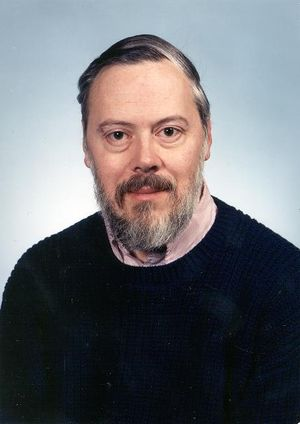
\includegraphics[width=0.2\paperwidth]{resources/dennis}
  	};
  	\end{tikzpicture}
  \end{frame}
  \begin{frame}{Introdução}
  	\framesubtitle{Nosso compilador}
  	\begin{itemize}
  		\item Dev-C++
  		\begin{itemize}
  			\item Ambiente de Desenvolvimento Integrado (IDE)
  			\item Contém o compilador GCC
  			\item Suporta C e C++
  			\item Gratuito e fácil de instalar
  			\item http://www.bloodshed.net/devcpp.html
  		\end{itemize}
  		\item Outras opções:
		\begin{itemize}
			\item Code::Blocks (http://www.codeblocks.org/)
			\item Microsoft Visual Studio (https://www.visualstudio.com/)
			\item GCC via Cygwin (http://www.cygwin.com/ - avançado)
		\end{itemize}
  	\end{itemize}
  \end{frame}
\begin{frame}[fragile]{Introdução}
 	\framesubtitle{Olá, mundo!}
 	\only<1>{\inputminted{c}{resources/helloworld.c}}
 	\only<2>{\inputminted[highlightlines=1]{c}{resources/helloworld.c}
	 	Inclusão de \texttt{stdio.h} da biblioteca padrão.
 	}
 	\only<3>{\inputminted[highlightlines=3]{c}{resources/helloworld.c}
	 	O programa começa a executar daqui.
 	}
 	\only<4>{
 		\inputminted[highlightlines=4]{c}{resources/helloworld.c}
 		Textos entre aspas são chamados de \alert{strings}. (O que é \textbf{\textbackslash n}?)
 	}
 	\only<5>{
 		\inputminted[highlightlines=5]{c}{resources/helloworld.c}
 		Terminamos a execução. Zero indica que tudo correu bem.
 	}
\end{frame}
\begin{frame}[fragile]{Introdução}
	\framesubtitle{Caracteres especiais}
	Alguns caracteres em uma string tem representação especial chamada \alert{sequência de escape}.
	
	\begin{exampleblock}{Errado}
		\inputminted{c}{resources/linebreakwrong.c}
	\end{exampleblock}
	\begin{exampleblock}{Correto}
		\inputminted{c}{resources/linebreakcorrect.c}
	\end{exampleblock}
\end{frame}
\begin{frame}{Introdução}
	\framesubtitle{Caracteres especiais}
	Principais sequências de escape em C:
	\begin{table}[!b]
	 {\carlitoTLF
	 \begin{tabularx}{\textwidth}{Xc}
	   \textbf{Caractere} & \textbf{Sequência de escape} \\
	   \toprule
	   Quebra de linha       & \textbackslash n \\
	   Retorno de carro      & \textbackslash r \\
	   Tabulação             & \textbackslash t \\
	   Contra-barra          & \textbackslash \textbackslash \\
	   Aspas duplas          &\textbackslash "  \\
	   \bottomrule
	 \end{tabularx}}
	\end{table}
\end{frame}
\begin{frame}[fragile]{Introdução}
	\framesubtitle{Caracteres especiais}
	\inputminted{c}{resources/escapes.c}
	\begin{block}{Saída}
		\inputminted{text}{resources/escapesout.txt}
	\end{block}
\end{frame}
\begin{frame}[fragile]{Introdução}
	\framesubtitle{Comentários}
	\only<1>{\inputminted{c}{resources/comments.c}}
	\only<2>{\inputminted[highlightlines=3-4]{c}{resources/comments.c}}
	\only<3>{\inputminted[highlightlines=6]{c}{resources/comments.c}}
\end{frame}

\section{Variáveis}
\begin{frame}[fragile]{Variáveis}
	\framesubtitle{Tipos}
	\inputminted{c}{resources/variable.c}
	\begin{figure}
	\begin{tikzpicture}
	\node at (0,0) {
		
\includegraphics[width=4.5cm]{resources/envelope}
	};
	\node at (0,1) {
		\LARGE 27
	};
	\node at (0,-1.4) {
		\Large \texttt{idade}
	};
	\end{tikzpicture}
	\end{figure}
\end{frame}
\begin{frame}{Variáveis}
	\framesubtitle{Tipos}
	Diversos tamanhos, chamados de \alert{tipos}:
	\begin{itemize}
		\item [\texttt{int}] Números inteiros. Em geral, pode armazenar valores de -2.147.483.648 até 2.147.483.647.
		\item [\texttt{char}] Geralmente utilizado para armazenar caracteres. Valores de -128 a 127.
		\item [\texttt{float}] Números decimais. Valores entre $\pm 3.4 \cdot 10^{\pm38}$ com cerca de 7 casas decimais.
		\item [\texttt{double}] Números decimais de precisão dupla. Valores entre $\pm 1.7 \cdot 10^{\pm308}$ com cerca de 15 casas decimais.
	\end{itemize}
\end{frame}
\begin{frame}{Variáveis}
	\framesubtitle{Tipos}
	Outros tipos:
	\begin{itemize}
		\item [\texttt{short}] Números inteiros, valores entre -32.768 e 32.767.
		\item [\texttt{long}] Números inteiros, valores entre -9.223.372.036.854.775.808 e 9.223.372.036.854.775.807.
	\end{itemize}
	O modificador \alert{\texttt{unsigned}} cria uma variável que só armazena números positivos (somente tipos inteiros).
	
	\texttt{char}: -128 a 127 $\Rightarrow$ \texttt{unsigned char}: 0 a 255
	
	Todos esses valores podem variar dependendo da plataforma.
	\pause
	\begin{tikzpicture}[overlay, remember picture]
	\node[anchor=center] at (current page.center) {
		
\includegraphics[width=0.7\paperwidth]{resources/nazare}
	};
	\end{tikzpicture}
\end{frame}
\begin{frame}{Variáveis}
	\framesubtitle{Tipos}
	Regra geral:
	\begin{itemize}
		\item Use \alert{\texttt{int}} para números inteiros.
		\item Use \alert{\texttt{char}} para caracteres.
		\item Use \alert{\texttt{double}} para números decimais.
	\end{itemize}
	
	\pause
	Por que não \alert{\texttt{double}} para tudo?
	\pause
	\begin{itemize}
		\item Operações com números decimais são mais lentas
		\item Erros de arredondamento
	\end{itemize}
\end{frame}
\begin{frame}{Variáveis}
	\framesubtitle{Identificadores}
	Os nomes dados às variáveis são chamados de \alert{identificadores}.
	
	Regras para os identificadores:
	\begin{itemize}
		\item Começar com uma letra ou underscore (\_)
		\item Os próximos caracteres podem ser letras, números ou underscores
		\item Não devem ser palavras reservadas (\texttt{return}, \texttt{int}, ...)
	\end{itemize}
	Use \textbf{nomes bem descritivos} para suas variáveis (prefira \alert{\texttt{altura}} em vez de \alert{\texttt{a}});
\end{frame}
\begin{frame}[fragile]{Variáveis}
	\framesubtitle{Exibição}
	\inputminted{c}{resources/showvars.c}
	\begin{block}{Saída}
		\inputminted{text}{resources/showvarsout.txt}
	\end{block}
\end{frame}
\begin{frame}{Variáveis}
	\framesubtitle{Exibição}
	\begin{table}[!b]
		{\carlitoTLF
			\begin{tabularx}{\textwidth}{Xc}
				\textbf{Tipo} & \textbf{Exibição} \\
				\toprule
				\texttt{int}               & \%d \\
				\texttt{unsigned int}      & \%u \\
				\texttt{float}             & \%f \\
				\texttt{double}            & \%lf \\
				\texttt{char}              & \%c  \\
				\texttt{long}              & \%ld  \\
				\texttt{unsigned long}     & \%lu  \\
				\bottomrule
			\end{tabularx}}
		\end{table}
		\pause
		E o caractere \alert{\%}? \pause Usamos \alert{\texttt{\%\%}}.
\end{frame}
\begin{frame}{Variáveis}
	\framesubtitle{Exibição}
	\begin{block}{Saída}
		\inputminted{text}{resources/showvarsout.txt}
	\end{block}
	Como esconder esses zeros?
\end{frame}
\begin{frame}[fragile]{Variáveis}
	\framesubtitle{Exibição}
	\only<1>{\inputminted{c}{resources/decimalplaces.c}}
	\only<2>{\inputminted[highlightlines=2]{c}{resources/decimalplaces.c}}
	\only<3>{\inputminted[highlightlines=3]{c}{resources/decimalplaces.c}}
	\only<4>{\inputminted[highlightlines=4]{c}{resources/decimalplaces.c}}
	\only<5>{\inputminted[highlightlines=5]{c}{resources/decimalplaces.c}}
	\begin{block}{Saída}
		\inputminted{text}{resources/decimalplaces.txt}
	\end{block}
\end{frame}
\section{Operações}
\begin{frame}{Operações}
	As principais operações matemáticas estão disponíveis:
	\begin{itemize}
		\item \textbf{Adição:} +
		\item \textbf{Subtração:} -
		\item \textbf{Multiplicação:} *
		\item \textbf{Divisão:} /
	\end{itemize}
	Valem as regras de precedência da matemática:
	\begin{enumerate}
		\item Multiplicações e divisões da esquerda para a direita
		\item Somas e subtrações da esquerda para a direita
	\end{enumerate}
\end{frame}
\begin{frame}{Operações}
	\inputminted{c}{resources/operations.c}
	\pause
	\begin{block}{Saída}
		\inputminted{text}{resources/operationsout.txt}
	\end{block}
\end{frame}
\begin{frame}{Operações}
	Podemos alterar a ordem das operações usando parênteses:
	\inputminted{c}{resources/parenthesis.c}
	\begin{block}{Saída}
		\inputminted{text}{resources/parenthesisout.txt}
	\end{block}
\end{frame}
\begin{frame}{Operações}
	A divisão entre dois inteiros será também inteira:
	\inputminted{c}{resources/division.c}
	\begin{block}{Saída}
		\inputminted{text}{resources/divisionout.txt}
	\end{block}
\end{frame}
\begin{frame}{Operações}
	O operator \alert{\texttt{\%}} calcula o resto da divisão:
	\inputminted{c}{resources/remainder.c}
	\begin{block}{Saída}
		\inputminted{text}{resources/remainderout.txt}
	\end{block}
\end{frame}
\begin{frame}{Operações}
	Este operador pode ser usado em operações de ``aritmética de relógio'':
	\inputminted{c}{resources/clock.c}
	\begin{block}{Saída}
		\inputminted{text}{resources/clockout.txt}
	\end{block}
\end{frame}
\begin{frame}{Operações}
	A biblioteca \alert{\texttt{math.h}} disponibiliza operações matemáticas:
	\begin{itemize}
		\only<1> {
			\item \textbf{Potenciação:} pow
			\item \textbf{Seno:} sin
			\item \textbf{Cosseno:} cos
			\item \textbf{Tangente:} tan
			\item \textbf{Raiz quadrada:} sqrt
			\item \textbf{Valor absoluto (inteiro):} abs
			\item \textbf{Valor absoluto (double):} fabs
		}
		\only<2>{
			\item \textbf{Logaritmo na base 10:} log10
			\item \textbf{Logaritmo natural:} log
			\item \textbf{Exponencial ($e^{x}$):} exp
			\item \textbf{Arredondamento para cima:} ceil
			\item \textbf{Arredondamento para baixo:} floor
			\item Dentre várias outras
		}
	\end{itemize}
\end{frame}
\begin{frame}{Operações}
	\only<1>{\inputminted{c}{resources/pithagoras.c}}
	\only<2>{\inputminted[highlightlines=2]{c}{resources/pithagoras.c}}
	\begin{block}{Saída}
		\inputminted{text}{resources/pithagorasout.txt}
	\end{block}
\end{frame}
\section{Entrada de dados}
\begin{frame}{Entrada de dados}
	A principal função que usaremos é a \alert{\texttt{scanf}}.
	\only<1>{\inputminted{c}{resources/scanf.c}}
	\only<2>{\inputminted[highlightlines=3]{c}{resources/scanf.c}}
	\begin{block}{Saída}
		\inputminted{text}{resources/scanfout.txt}
	\end{block}
\end{frame}
\begin{frame}{Entrada de dados}
	Importante lembrar sobre a \texttt{scanf}:
	\begin{itemize}
		\item Utiliza os mesmos especificadores que vimos na \texttt{printf}
		\item Lembrar sempre de colocar o \alert{\texttt{\&}} antes do nome da variável (entenderemos o motivo mais adiante)
	\end{itemize}
\end{frame}
\section{Exercícios}
\begin{frame}{Exercícios}
	\framesubtitle{Exercício 1}
	Escreva um programa que imprima seu nome na tela. Cada nome deve estar em uma linha separada.
\end{frame}
\begin{frame}{Exercícios}
	\framesubtitle{Exercício 1}
	\inputminted{c}{resources/ex1.c}
\end{frame}
\begin{frame}{Exercícios}
	\framesubtitle{Exercício 2}
	Escreva um programa que calcule o valor de:
	\begin{equation}
		\frac{26+2\cdot 5}{(7+2)\cdot 4}
	\end{equation}
\end{frame}
\begin{frame}{Exercícios}
	\framesubtitle{Exercício 2}
	\inputminted{c}{resources/ex2.c}
\end{frame}
\begin{frame}{Exercícios}
	\framesubtitle{Exercício 3}
	Escreva um programa que receba um número pelo teclado e eleve o número ao quadrado.
\end{frame}
\begin{frame}{Exercícios}
	\framesubtitle{Exercício 3}
	\inputminted{c}{resources/ex3.c}
\end{frame}
\begin{frame}{Exercícios}
	\framesubtitle{Exercício 4}
	Marina acaba de comprar um carro. O pagamento será feito da seguinte maneira:
	\begin{itemize}
		\item 40\% do valor a vista
		\item O restante dividido em 10 parcelas
	\end{itemize}
	Escreva um programa que receba o valor do carro pelo teclado e imprima o valor a ser pago à vista e o valor de cada parcela.
\end{frame}
\begin{frame}{Exercícios}
	\framesubtitle{Exercício 4}
	\inputminted[fontsize=\small]{c}{resources/ex4.c}
\end{frame}
\end{document}
